\chapter{RESULT AND DISCUSSION}


\section{Experiment Setup}
All experiments were conducted on Kaggle's cloud-based GPU infrastructure.
Table~\ref{tab:hardware} summarises the hardware and software environment used
throughout training and evaluation.
 
\begin{table}[h!]
\centering
\renewcommand{\arraystretch}{1.1} 
%\large
\begin{tabular}{|l|l|}
\hline
\textbf{Component} & \textbf{Specification} \\ \hline
GPU                      & NVIDIA Tesla T4 (16 GB VRAM) \\ \hline
System RAM               & 29 GB \\ \hline
Operating System         & Linux (Ubuntu 20.04) \\ \hline
Python                   & 3.10 \\ \hline
PyTorch                  & 2.1 (CUDA 12.1) \\ \hline
HuggingFace Transformers & 4.40 \\ \hline
Training Precision       & fp16 (mixed precision) \\ \hline
Training Platform        & Kaggle Notebooks \\ \hline
\end{tabular}
\vspace{2pt} % Adds a small gap between table and caption
\caption{Hardware and software environment}
\label{tab:hardware}
\end{table}

\section{Training Configuration}

Four model configurations were explored during the course of this project,each differing in encoder backbone and decoder architecture.

\noindent The Baseline model retained the original RoBERTa-based decoder from microsoft/trocr-base-handwritten with the Devanagari character set
added to its existing vocabulary. While this required minimal changes, the RoBERTa decoder had been pre-trained on English text, causing it to treat
Devanagari characters as rare multi-byte fallback tokens and producing excessively long, fragmented token sequences with poor generation coherence for Nepali words.

\noindent The TrOCR-Small variant replaced the ViT-Base encoder with a ViT-Small encoder of approximately 22 million parameters. Although this reduced memory usage and training time, the smaller encoder capacity limited the richness of visual features available for structurally complex conjunct consonants and compound Devanagari characters, resulting in higher recognition errors on difficult word forms.

\noindent The TrOCR-Large variant used a ViT-Large encoder with 307 million parameters across 24 transformer layers, paired with a larger custom BERT
decoder of 4 layers and 8 attention heads. While the larger encoder provided richer visual representations, the substantially increased memory footprint made full Phase~2 fine-tuning impractical on the available Kaggle GPU infrastructure, restricting the number of training epochs and limiting the model's final performance.
 
\noindent Based on these observations, the Proposed Model~(v3) was selected as the primary configuration. It pairs the ViT-Base encoder which provides sufficient visual representation capacity for Devanagari handwriting without the memory constraints of the large variant along with a compact custom BERT-based decoder of only 2 transformer layers, 4 attention heads, and a hidden dimensionality of 256, yielding approximately 4 million decoder parameters. This lightweight decoder was intentionally designed to avoid overfitting on the approximately 70,000 training samples while retaining sufficient capacity for character-level autoregressive generation.
Crucially, replacing the English-pretrained RoBERTa decoder with a custom character-level decoder built entirely from the Devanagari vocabulary eliminates the tokenizer mismatch present in the baseline, achieving complete character coverage with zero unknown token occurrences. The proposed model therefore offers the best balance of recognition accuracy,training efficiency, and stability under the available computational constraints, and is the focus of the evaluation presented in this chapter.
Quantitative results for all four variants are reported in
Table~\ref{tab:model_variants}.
\begin{table}[H]
\centering
\vspace{8pt}
\renewcommand{\arraystretch}{1.4}
%\large 
\begin{tabular}{|l|l|}
\hline
\textbf{Training Setting} & \textbf{Value (all variants)} \\ \hline
Dataset                  & IIIT-HW-Dev \\ \hline
Train / Val / Test       & 69,802 / 12,713 / 12,865 images \\ \hline
Tokenizer                & Custom Devanagari (112 tokens) \\ \hline
Loss function            & Label-smoothed CE ($\alpha = 0.1$) \\ \hline
Optimiser                & AdamW ($\beta_1=0.9, \beta_2=0.999$) \\ \hline
Batch size (effective)   & 32 (micro-batch 8, accumulation 4) \\ \hline
Mixed precision          & fp16 \\ \hline
Decoding (inference)     & Beam search (\texttt{num\_beams} $= 4$) \\ \hline
Evaluation metrics       & CER, WER, Accuracy \\ \hline
Training platform        & Kaggle (NVIDIA Tesla T4) \\ \hline
\end{tabular}
\caption{Shared training configuration across all model variants}
\label{tab:shared_config}
\end{table}

\begin{table}[H]
\centering
\vspace{8pt}
\renewcommand{\arraystretch}{1.9}
\begin{tabular}{|p{2.4cm}|p{1.8cm}|p{3.2cm}|p{1.8cm}|c|c|c|}
\hline
\textbf{Model} & \textbf{Encoder} & \textbf{Decoder} & \textbf{Dec. Prm} & \textbf{CER\%} & \textbf{WER\%} & \textbf{Acc.\%} \\ \hline
Baseline & ViT-Base & RoBERTa (ext) & $\sim$125M & 41.92 & 52.92 & 57.49 \\ \hline
TrOCR-Small & ViT-Small & Custom (2L/4H) & $\sim$4M & 13.29 & 29.7 & 70.13 \\ \hline
TrOCR-Large & ViT-Large & Custom (4L/8H) & $\sim$13M & 8.08& 20.40 & 79.60 \\ \hline
\textbf{Proposed TrOCR base with custom decoder} & \textbf{ViT-Base} & \textbf{Custom BERT} & \textbf{$\sim$4M} & \textbf{5.43} & \textbf{16.58} & \textbf{83.42} \\ \hline
\end{tabular}
\caption{Architectural comparison and test set results across all model variants}
\label{tab:model_variants}
\end{table}

\subsection{TrOCR base Model Results}
The training process was conducted in two distinct phases. During Phase 1 (epochs 1–15), the Vision Transformer (ViT) encoder remained frozen, and only the custom decoder which was configured with 2 layers, 4 attention heads, and a hidden dimension of 256 was trained. As a result, the Character Error Rate (CER) initially remained relatively high (approximately 21\%) and exhibited fluctuations. This behavior can be attributed to the decoder learning from scratch while relying on fixed visual representations that were not specifically optimized for the target task. The temporary increase in CER observed around epochs 12–13 (rising from 16.8\% to 21.4\%) reflects a common phenomenon in training dynamics, where the model departs from a local optimum before converging toward a more effective solution.

\noindent Phase 2 began at epoch 16, when the encoder was unfrozen and allowed to fine-tune jointly with the decoder. This transition resulted in a noticeable improvement in performance, with CER decreasing sharply from approximately 11.7\% to 10\% within a few epochs. The improvement is explained by the encoder adapting its feature representations;which was originally trained on English handwriting using TrOCR for better capturing of the structural characteristics of the Devanagari script, including its distinctive stroke patterns and vowel diacritics (matras). Following this adjustment, both encoder and decoder components converged more effectively, leading to a steady decline in CER.

\noindent From epoch 16 onward, the gradual and consistent reduction in CER, ultimately reaching a minimum value of 6.68\% at epoch 52, indicates stable learning. The absence of abrupt fluctuations during this phase suggests that the learning rate strategy ; Cosine Annealing with Warm Restarts was appropriately conservative. This choice helped maintain stability during fine-tuning, preventing disruption of the pretrained encoder weights while enabling continuous performance improvements.

\noindent Figure~\ref{fig:training_curves} illustrates the progression of training loss and validation Character Error Rate (CER) across epochs, highlighting the performance improvement following encoder unfreezing at epoch 16.
\begin{figure}[h]
    \centering

    \begin{subfigure}[b]{0.48\textwidth}
        \centering
        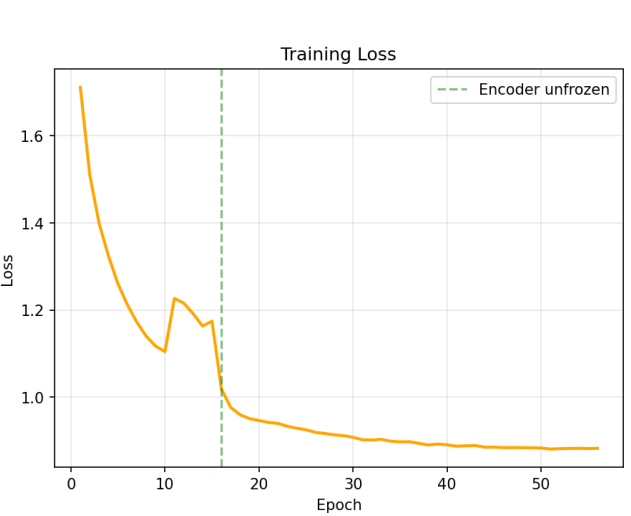
\includegraphics[width=\textwidth]{img/train_loss.png}
        \caption{Train loss vs Epoch}
        \label{fig:train_loss}
    \end{subfigure}
    \hfill                                              
    \begin{subfigure}[b]{0.48\textwidth}
        \centering
        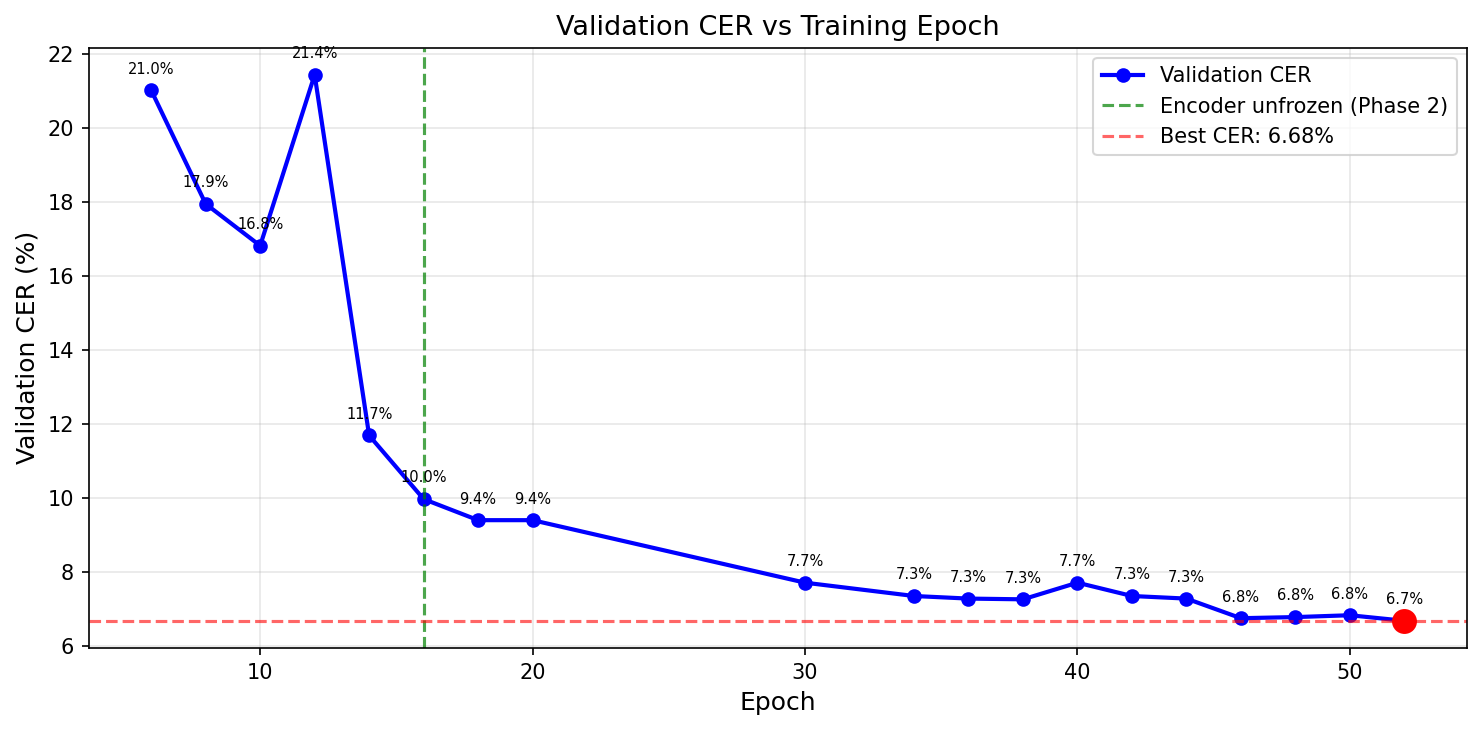
\includegraphics[width=\textwidth]{img/Val_cer.png} 
        \caption{Validation CER vs Epoch}
        \label{fig:val_cer}
    \end{subfigure}

    \caption{Training dynamics across epochs. The green dashed line marks the transition to Phase 2 (encoder unfrozen). The red dashed line indicates the best validation CER of 6.68\%.}
    \label{fig:training_curves}
\end{figure}


\newpage
\noindent The distribution of Normalized Edit Distance (NED) is highly right-skewed, indicating that the model performs very well on the majority of test samples while struggling with a small subset of more difficult cases. A total of 10,736 samples, representing approximately 83.5\% of the test set, achieved perfect recognition (NED = 0). This large concentration at zero demonstrates that the model is able to accurately predict most words without any character-level errors.

\noindent Despite this strong performance, the mean NED is 5.22\%, which is slightly elevated due to a small number of challenging samples forming a long, sparse tail in the distribution. These outliers correspond to cases where the model makes significant errors, including instances where predictions are entirely incorrect (NED = 100\%). However, such cases are relatively rare and do not substantially affect the overall performance trend.

\noindent Normalized Edit Distance is defined as the edit distance divided by the maximum length of the predicted and reference sequences. Unlike Character Error Rate (CER), which normalizes only by the reference length, NED accounts for both insertions and deletions more symmetrically by penalizing predictions that are excessively longer or shorter than the ground truth. In this evaluation, the NED (5.22\%) and CER (5.82\%) values are very close, suggesting that the model maintains good control over sequence length. In other words, it is neither frequently generating extra characters nor truncating outputs, which indicates stable and well-calibrated predictions.

\noindent Overall, the distribution reflects a model that is highly accurate on most inputs, with only a small proportion of difficult cases contributing to the residual error.
\begin{figure}[H]
    \centering
    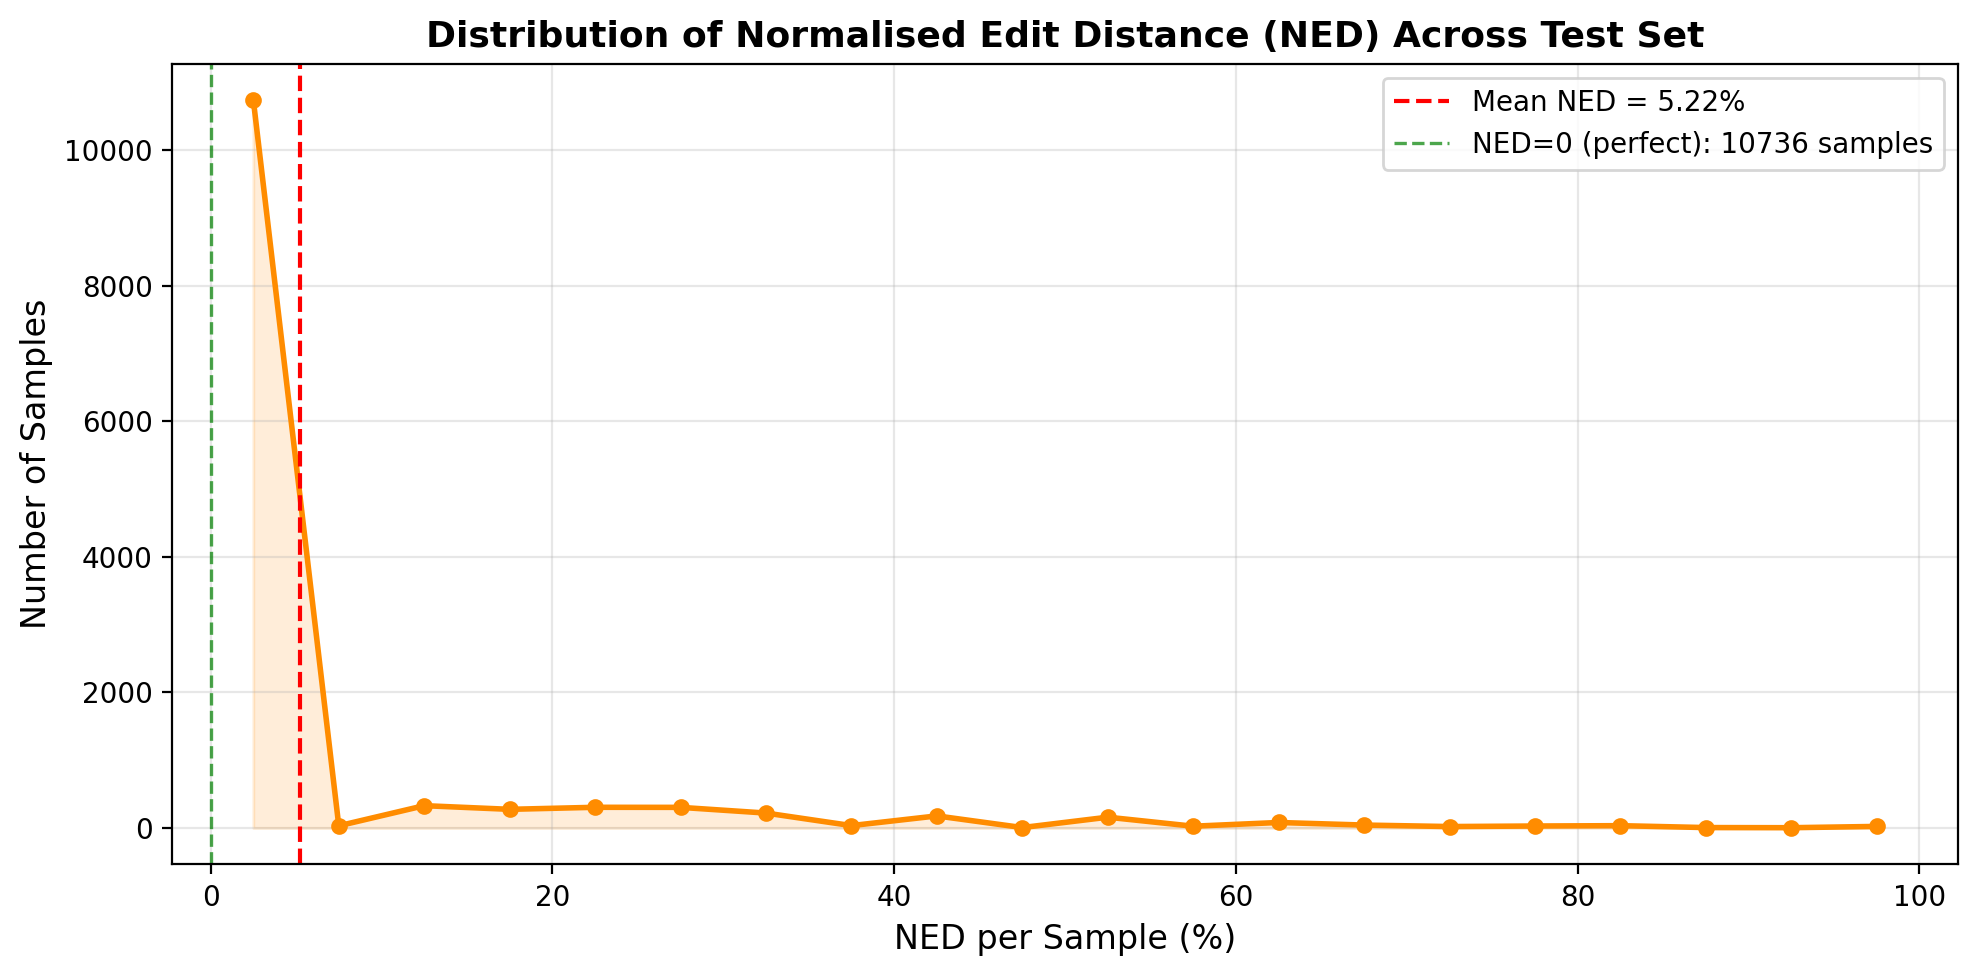
\includegraphics[width=0.85\textwidth]{img/metric_ned_distribution.png}
    \caption{Distribution of Normalised Edit Distance (NED) scores across the test set.}
    \label{fig:ned_dist}
\end{figure}
\newpage
\noindent Similarly, the cumulative accuracy analysis shows a steep and consistent improvement as the tolerance for character-level errors increases. At zero tolerance (K = 0), 83.5\% of the predictions are exactly correct, indicating a strong baseline performance. When a tolerance of one character error is allowed (K = 1), the accuracy rises significantly to 92.4\%, and further increases to 98.1\% by K = 3. Overall, the accuracy reaches 96.0\% within just two character errors, demonstrating that the majority of model predictions are very close to the ground truth.

\noindent This trend indicates that most of the model’s errors are minor, typically involving only one or two incorrect characters, rather than large or completely incorrect predictions. Such behavior suggests that the model is generally reliable and rarely produces catastrophic errors.

\noindent From an application perspective, this is a particularly strong result. In practical OCR systems integrated with downstream natural language processing tasks, small character-level errors are often recoverable through post-processing techniques such as spell-checking or language model correction. Therefore, even when the model does not achieve perfect predictions, its outputs remain highly usable and can be refined further with minimal effort.
\begin{figure}[H]
    \centering
    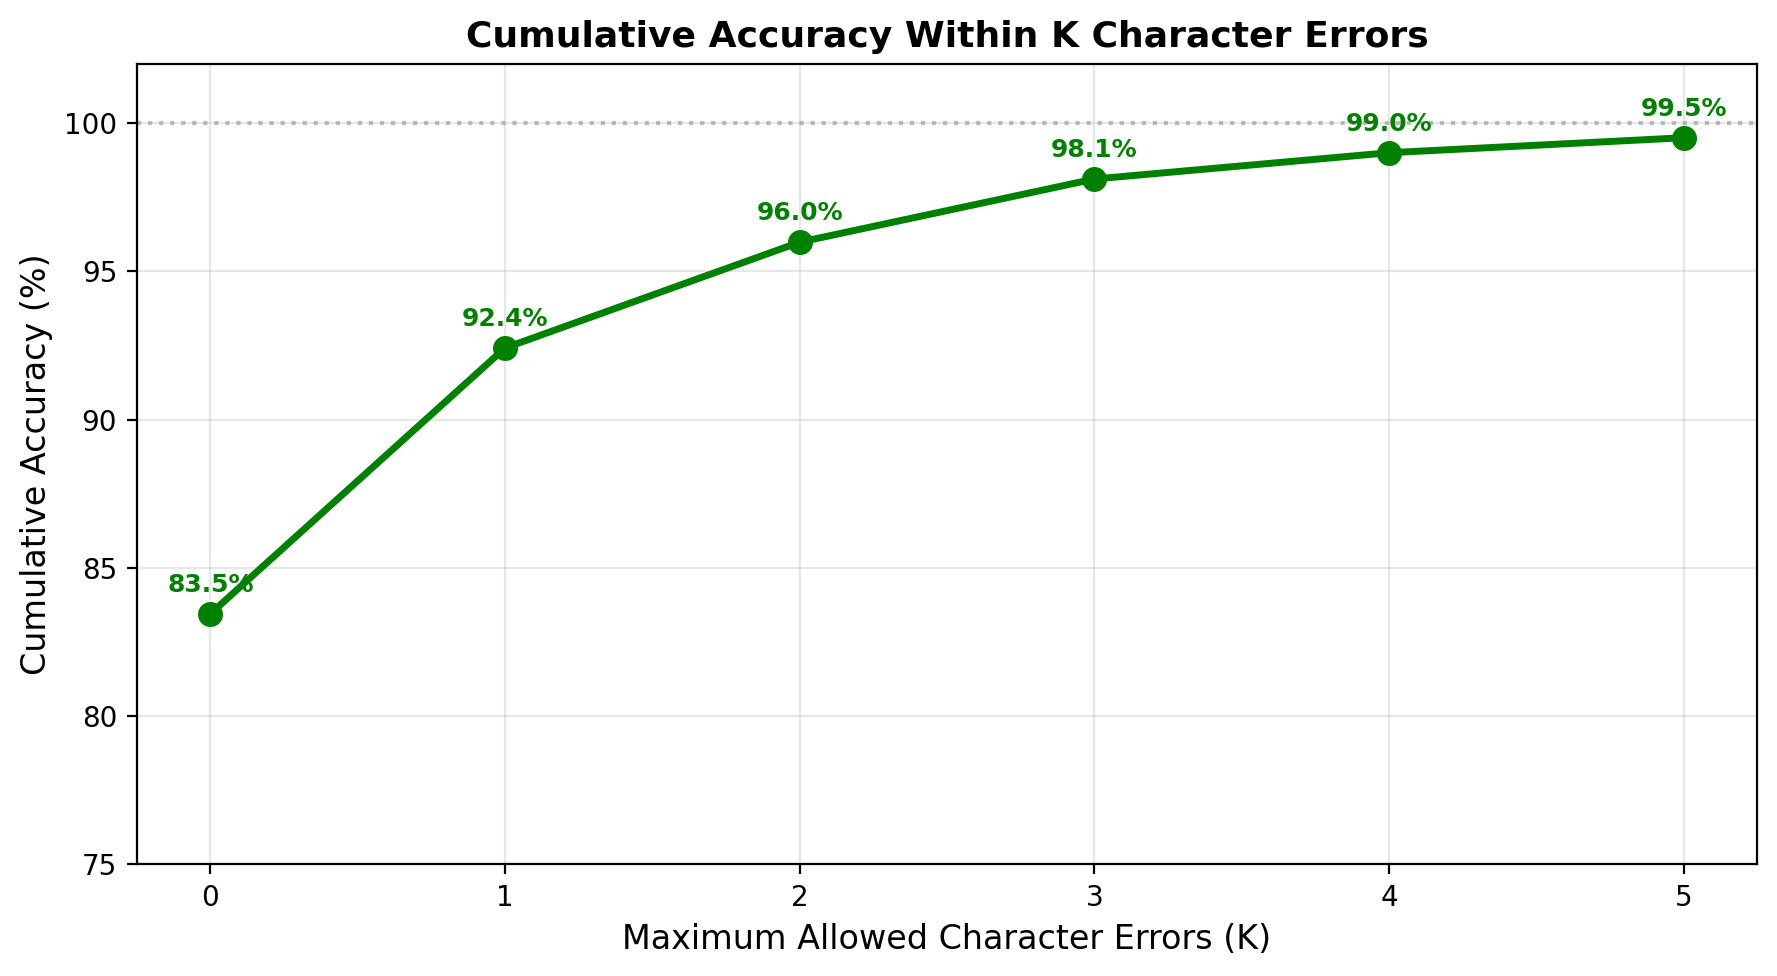
\includegraphics[width=0.85\textwidth]{img/metric_cumulative_accuracy.png}
    \caption{Cumulative accuracy within $K$ character errors.}
    \label{fig:cumulative_acc}
\end{figure}
\newpage
\noindent The evaluation of model performance across varying word lengths indicates that exact match accuracy remains relatively stable, ranging between 82\% and 85\% for words comprising 2 to 11 characters. In contrast, the Character Error Rate (CER) exhibits a pronounced decline as word length increases. This inverse relationship reflects the reduced proportional impact of individual character errors in longer sequences, where isolated mistakes contribute less significantly to the overall error metric.

\noindent A consistent trend is observed for shorter to mid-length words (lengths 1–9), where CER decreases substantially from approximately 29\% to around 4\%. This behavior is expected, as longer words provide increased contextual and structural information, enabling more reliable pattern recognition. Conversely, shorter words, particularly those consisting of one or two characters, present limited contextual cues and are therefore more susceptible to misclassification.

\noindent Variations in performance at higher word lengths, specifically at lengths 13 and 15, can be attributed primarily to limited sample sizes. With only 34 and 14 samples respectively, these categories are highly sensitive to the influence of a small number of difficult instances, resulting in noticeable fluctuations in both accuracy and CER. A similar phenomenon is observed at length 14, where accuracy reaches 89.5\% based on a sample size of 38, likely reflecting a relatively less challenging subset of data rather than a consistent performance improvement.

\noindent Performance degradation for very short words is particularly evident at length 1, where the dataset contains only 24 samples. In addition to the limited sample size, the inherent visual ambiguity of isolated Devanagari characters contributes to this effect. Characters combined with vowel diacritics (matras) often exhibit similar visual structures, and in the absence of surrounding context, the model faces increased difficulty in disambiguating such cases.
\begin{figure}[H]
    \centering
    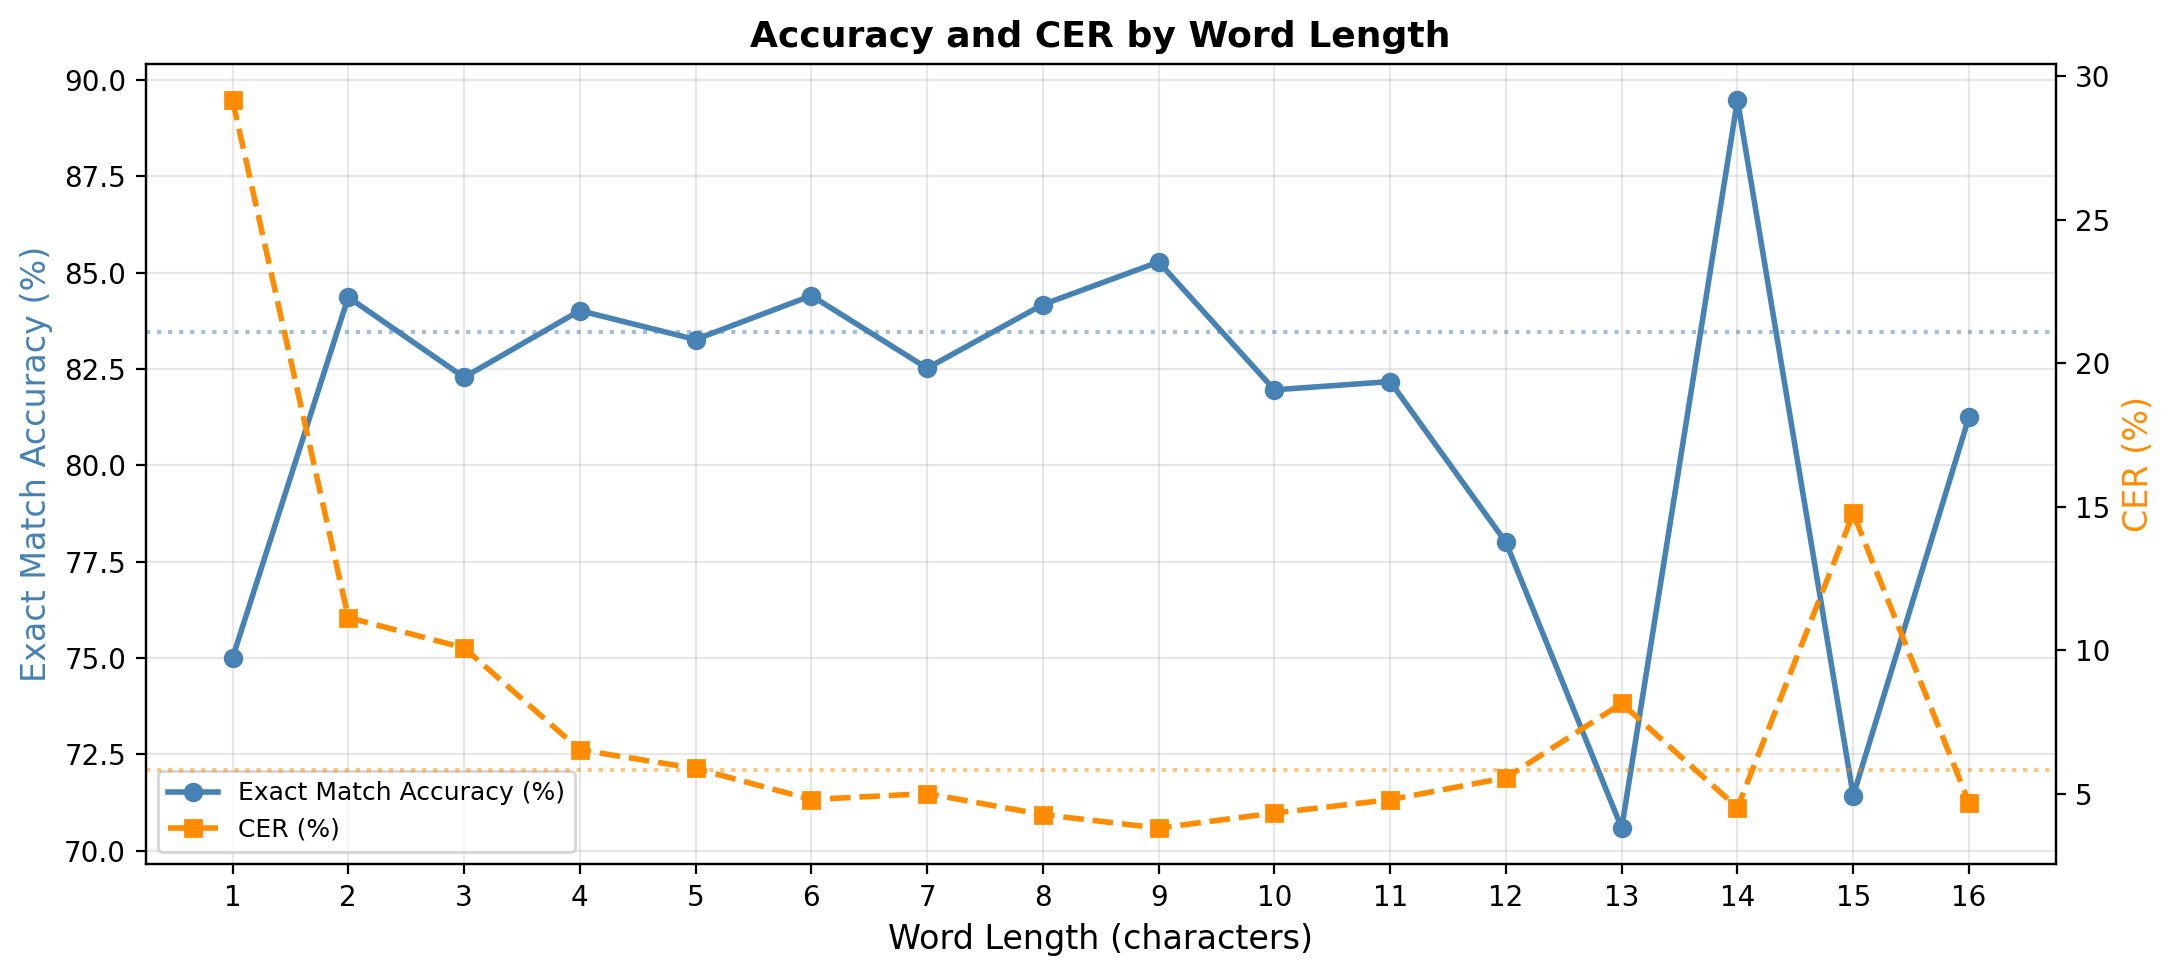
\includegraphics[width=0.85\textwidth]{img/metric_by_word_length.png}
    \caption{Exact Match Accuracy and CER as a function of word length.}
    \label{fig:by_length}
\end{figure}

\noindent Overall, The model achieves a CER of 5.82\%, WER of 16.55\%, NED of 5.22\%, exact-match accuracy of 83.45\%, and 1-NED of 94.78\%, collectively demonstrating strong character-level recognition with moderate word-level precision.
\begin{figure}[H]
    \centering
    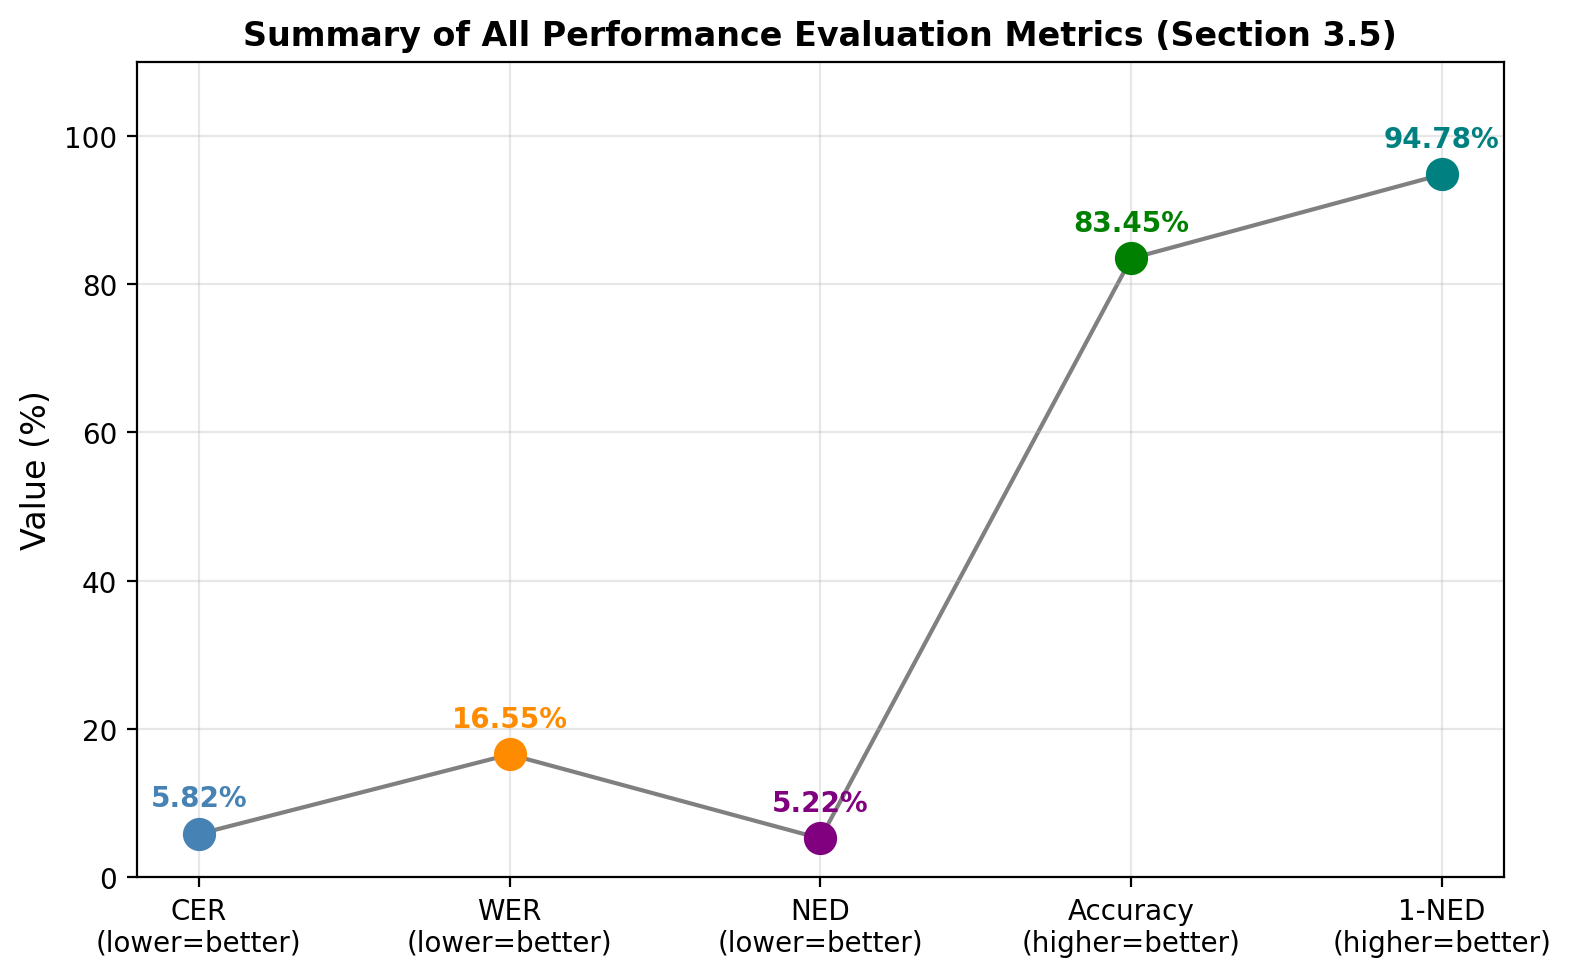
\includegraphics[width=0.75\textwidth]{img/metric_summary_all.png}
    \caption{Summary of all performance evaluation metrics (Section~3.5).}
    \label{fig:metric_summary}
\end{figure}


\newpage
\section{Software Development Approach}
\noindent Agile development methodology is a quick and flexible iterative development methodology for software development. It divides work into manageable chunks without requiring a lot of advance planning. The needs and scope of the project are established early on, and iterations are planned. A functioning product demo is the end result of each iteration, which includes all phases of the software development life cycle: planning, requirements analysis, design, coding, and testing. By iteratively improving the product in response to feedback, this methodology lowers project risk and speeds up delivery overall.
    \begin{figure}[H]
        \centering
        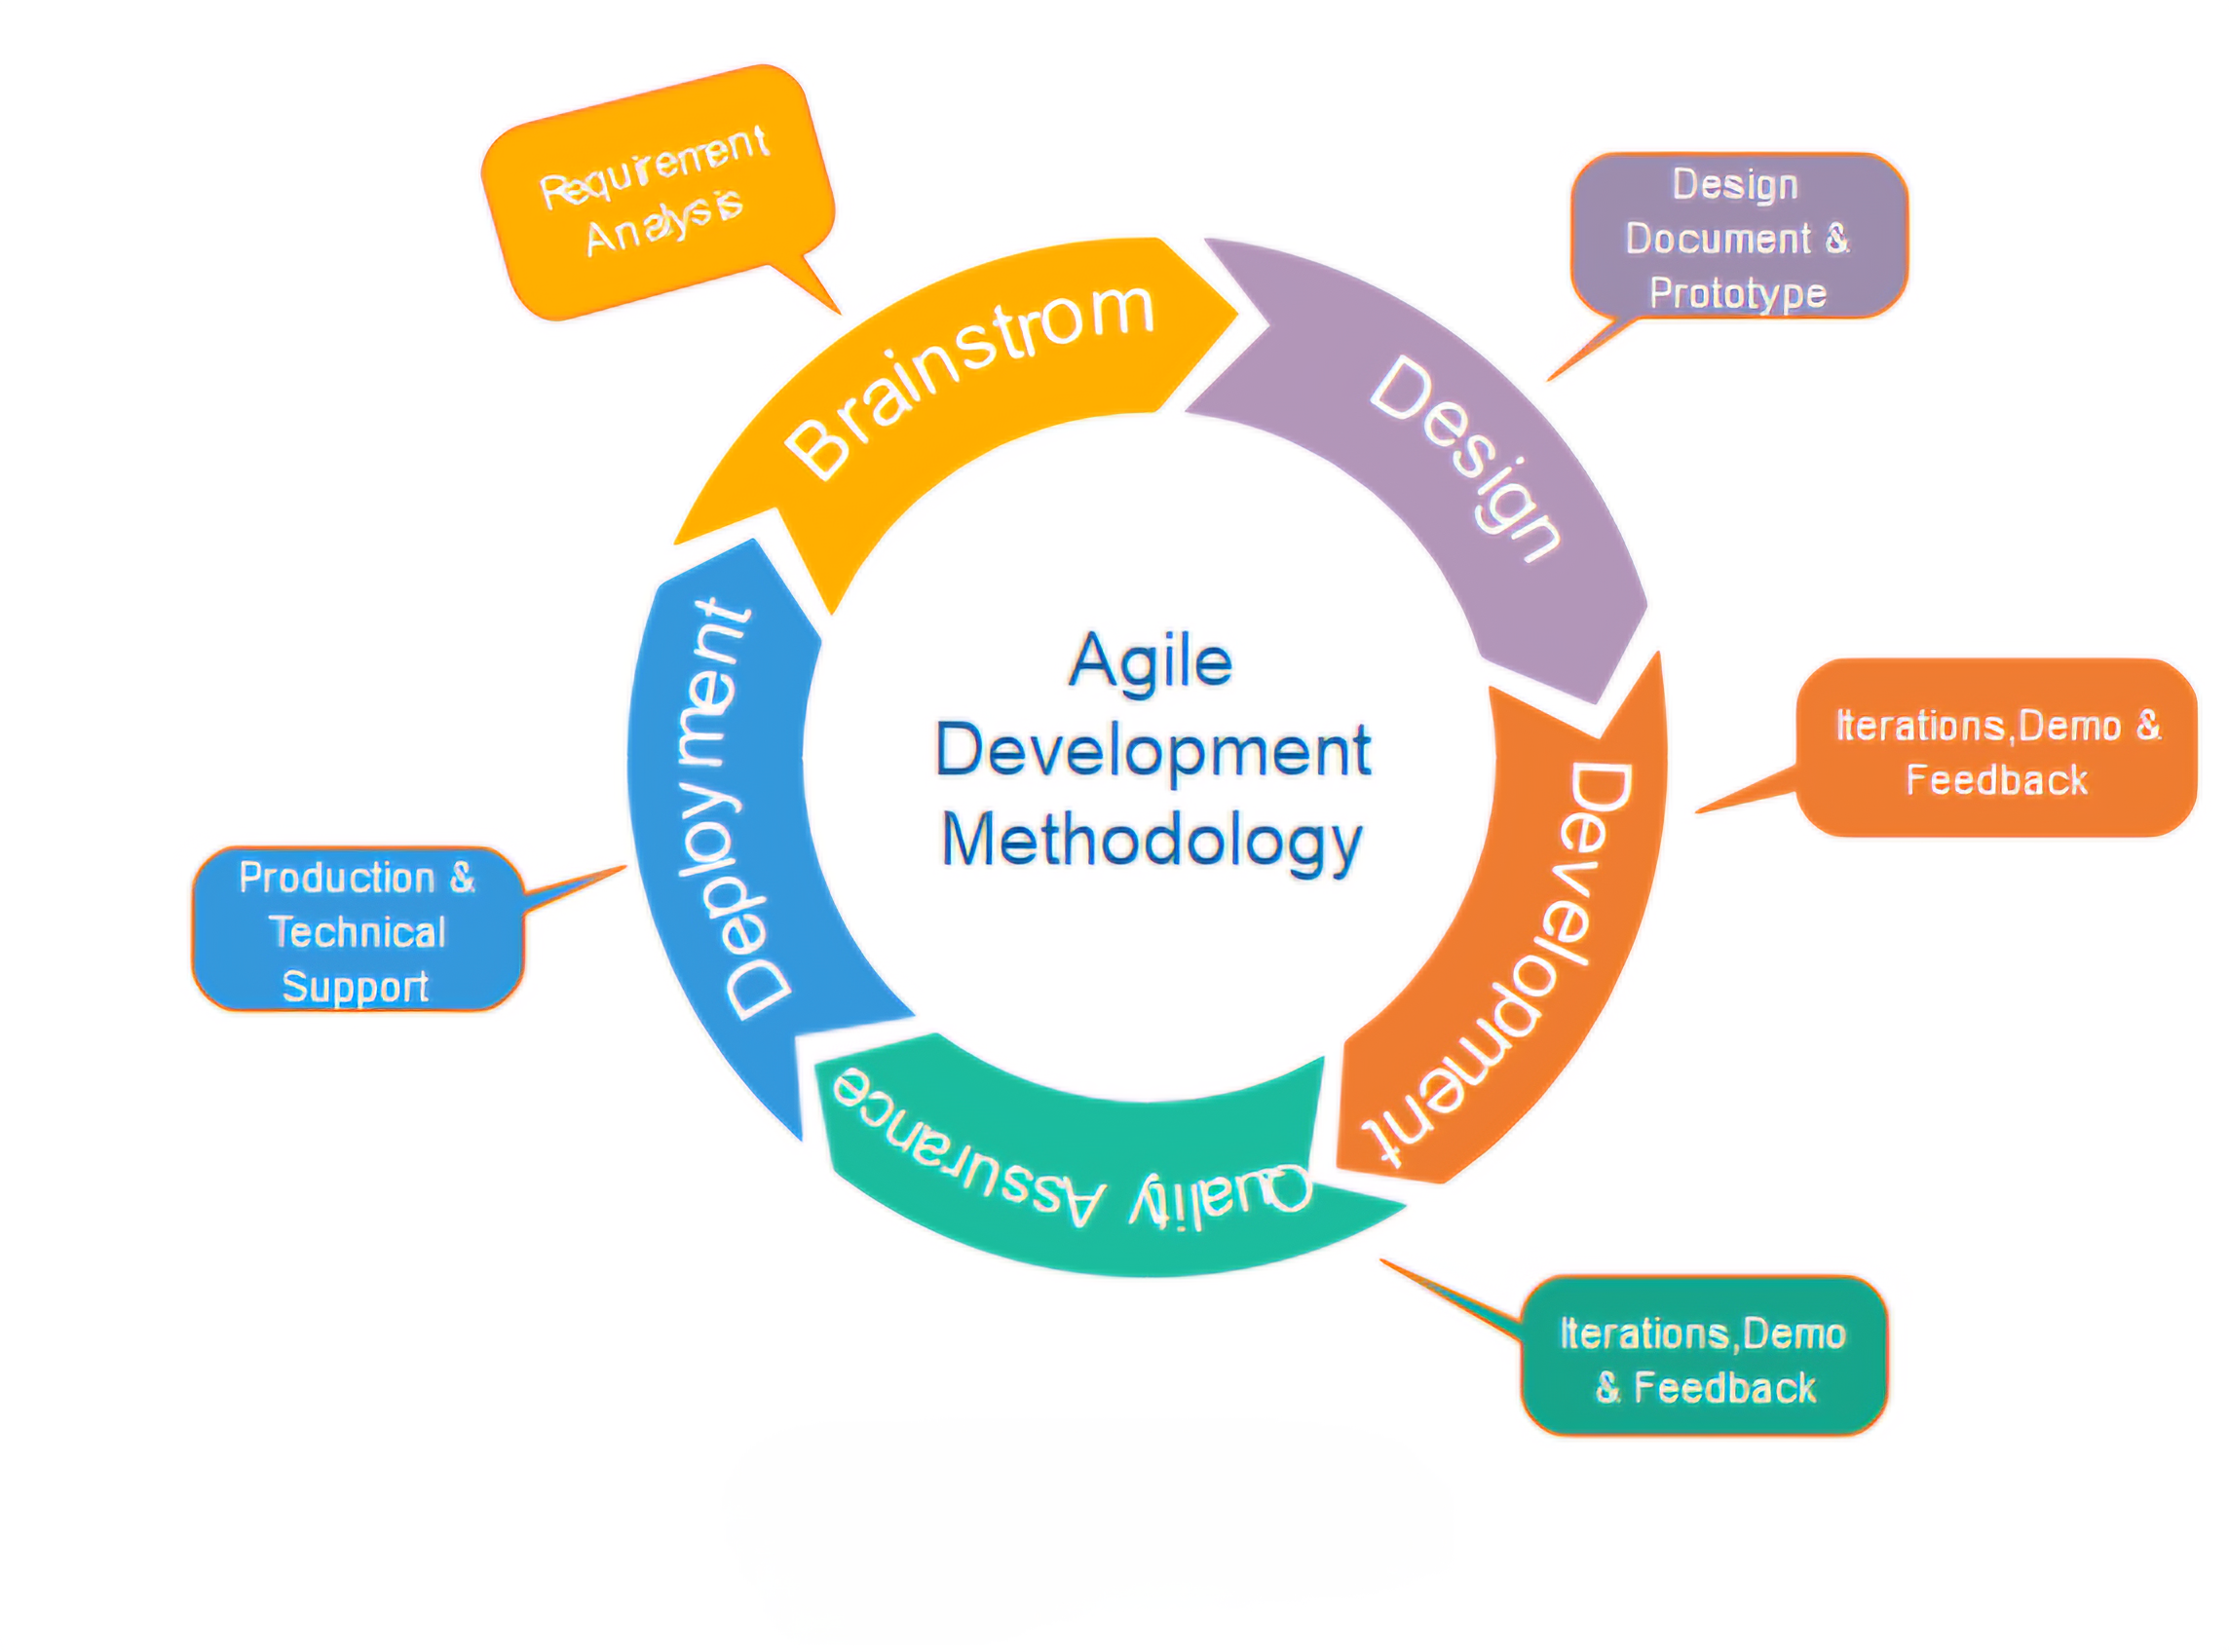
\includegraphics[scale=0.1]{img/agilemodel.png}
        \caption{Agile Development Model}
        \label{fig:agilemodel}
    \end{figure}
\subsection{Agile Sprints}

\subsubsection{Sprint 1: Dataset Acquisition and Initial Exploration}
\textbf{Duration:} Mid-December, Weeks 1--2\\
\textbf{Goal:} Identify and acquire a suitable dataset for handwritten Nepali word recognition and assess the feasibility of a character-level recognition approach.

\textbf{Key Activities:}
\begin{itemize}
    \item Surveyed publicly available Devanagari handwriting datasets and evaluated their suitability for word-level Nepali OCR.
    \item Acquired a Devanagari Character Dataset and manually curated 
    an additional matra (diacritic) dataset to supplement 
    underrepresented character classes.
    \item Implemented and tested an initial character-level recognition 
    pipeline to assess baseline feasibility.
    \item Identified critical limitations of the character-level 
    approach, including low accuracy and inadequate representation 
    of compound characters and matras.
    \item Collectively decided to abandon the character-level approach 
    in favour of word-level recognition based on evaluation outcomes.
\end{itemize}

\textbf{Outcomes:}
\begin{itemize}
    \item Character-level approach evaluated and rejected on accuracy 
    grounds.
    \item Decision made to adopt word-level recognition using a 
    dedicated word-image dataset.
    \item Clear direction established for Sprint 2.
\end{itemize}

\subsubsection{Sprint 2: Dataset Preparation and Pre-processing 
Pipeline}
\textbf{Duration:} Late December -- Early January, Weeks 3--5\\
\textbf{Goal:} Acquire the IIIT-HW-Dev word-level dataset, parse it 
into structured image--label pairs, and build a robust image 
pre-processing pipeline.

\textbf{Key Activities:}
\begin{itemize}
    \item Obtained the IIIT-HW-Dev dataset from Kaggle, comprising 
    95,380 segmented handwritten word images with Unicode labels, 
    and parsed it into training (69,802), validation (12,713), and 
    test (12,865) splits.
    \item Identified 108 unique Devanagari characters across the 
    dataset, with a maximum label length of 23 characters.
    \item Designed and implemented a multi-step image pre-processing 
    pipeline comprising grayscale conversion, Gaussian denoising, 
    adaptive binarisation, morphological closing, deskewing, tight 
    cropping, and letterbox padding to $128 \times 128$ pixels.
    \item Pre-cached all processed images to disk to avoid repeated 
    computation during training.
    \item Built and validated a custom character-level tokenizer with 
    a 112-token Devanagari vocabulary including four special tokens 
    (\texttt{<pad>}, \texttt{<s>}, \texttt{</s>}, \texttt{<unk>}).
\end{itemize}

\textbf{Outcomes:}
\begin{itemize}
    \item Fully parsed and split IIIT-HW-Dev dataset ready for 
    training.
    \item Pre-processing pipeline implemented, validated, and cached.
    \item Custom tokenizer built and smoke-tested on Devanagari 
    word samples.
\end{itemize}

\subsubsection{Sprint 3: Model Architecture Design and Initialisation}
\textbf{Duration:} January, Weeks 6--7\\
\textbf{Goal:} Design and initialise the encoder--decoder model 
architecture and configure the training infrastructure.

\textbf{Key Activities:}
\begin{itemize}
    \item Selected microsoft/trocr-base-handwritten as the 
    source of the pre-trained ViT encoder, leveraging its existing 
    fine-tuning on handwritten document images.
    \item Designed a lightweight custom BERT-based decoder with 2 transformer layers, 4 attention heads, hidden size 256, and FFN intermediate size 512 with approximately 4 million parameters that were sized appropriately for the training corpus.
    \item Integrated the encoder and decoder into a single end-to-end trainable model using HuggingFace's 
 VisionEncoderDecoderModel framework.
    \item Configured cross-attention between encoder and decoder, 
    token special IDs, and the data loading pipeline with on-the-fly 
    training augmentation (Gaussian blur, random affine, colour 
    jitter, random perspective, and random erasing).
    \item Set up mixed-precision training (fp16), gradient 
    accumulation over 4 steps, and automatic checkpoint uploading 
    to Kaggle every 2 epochs.
\end{itemize}

\textbf{Outcomes:}
\begin{itemize}
    \item Full model architecture designed and initialised.
    \item Training infrastructure configured and validated on a 
    small batch of training data.
    \item Data pipeline with augmentation confirmed operational.
\end{itemize}

\subsubsection{Sprint 4: Phase 1 Training -- Decoder-Only}
\textbf{Duration:} January -- February, Weeks 8--10\\
\textbf{Goal:} Train the decoder in isolation with the encoder frozen 
to establish baseline Devanagari text generation capability without 
disturbing pre-trained visual features.

\textbf{Key Activities:}
\begin{itemize}
    \item Froze all ViT encoder parameters and trained only the 
    decoder using AdamW with learning rate $5 \times 10^{-4}$ and 
    weight decay $10^{-3}$.
    \item Applied label-smoothed cross-entropy loss with smoothing 
    coefficient 0.1 and gradient clipping at norm 1.0.
    \item Monitored validation CER and WER every 2 epochs and saved 
    the best-performing checkpoint automatically.
    \item Observed steady reduction in validation CER across 
    training epochs, confirming that the decoder was successfully 
    learning Devanagari character generation patterns.
\end{itemize}

\textbf{Outcomes:}
\begin{itemize}
    \item Stable decoder-only baseline established.
    \item Best Phase 1 checkpoint saved for use in Phase 2.
    \item Validation CER and WER trends reviewed collectively to 
    inform Phase 2 training configuration.
\end{itemize}

\subsubsection{Sprint 5: Phase 2 Training -- Full Fine-Tuning}
\textbf{Duration:} February -- March, Weeks 11--14\\
\textbf{Goal:} Unfreeze the ViT encoder and fine-tune the entire 
model end-to-end to adapt visual features to handwritten Devanagari 
and further reduce CER.

\textbf{Key Activities:}
\begin{itemize}
    \item Unfroze the encoder and applied differential learning 
    rates: $5 \times 10^{-7}$ for the encoder and $5 \times 
    10^{-5}$ for the decoder, to prevent catastrophic forgetting 
    of pre-trained visual representations.
    \item Continued training with \texttt{CosineAnnealingWarmRestarts} 
    scheduler ($T_0 = 10$, $\eta_{\min} = 10^{-8}$) across multiple 
    Kaggle sessions, resuming from the latest checkpoint each time.
    \item Iteratively reviewed validation CER and WER at the end of 
    each session and adjusted hyperparameters accordingly.
    \item Achieved a best validation CER of 7.26\% over the course 
    of full fine-tuning.
    \item Applied early stopping with patience of 10 validation 
    rounds to prevent overfitting.
\end{itemize}
\newpage
\textbf{Outcomes:}
\begin{itemize}
    \item Best model checkpoint achieving 6.68\% CER saved for 
    evaluation.
    \item Full training completed across 52 epochs with early 
    stopping.
    \item Model confirmed stable and non-overfitting based on 
    train--validation loss gap monitoring.
\end{itemize}

\subsubsection{Sprint 6: Evaluation and Inference}
\textbf{Duration:} March, Weeks 15--16\\
\textbf{Goal:} Conduct final evaluation on the held-out test set, 
implement single-image inference with confidence scoring, and 
prepare the system for demonstration.

\textbf{Key Activities:}
\begin{itemize}
    \item Loaded the best model checkpoint and evaluated it on the 
    full test set of 12,865 word images using beam search 
    (num\_beams = 4).
    \item Computed CER, WER, and Exact Match Accuracy on the test 
    set after Unicode NFC normalisation of all predicted and 
    ground-truth strings.
    \item Implemented single-image inference with test-time 
    augmentation (TTA) across four image variants and confidence 
    scoring from beam sequence log-probabilities.
    \item Validated predictions qualitatively on sample test images 
    and batch inference grids.
    \item Compiled training curves, CER history, and sample 
    prediction outputs for inclusion in the project report.
\end{itemize}

\textbf{Outcomes:}
\begin{itemize}
    \item Final test set CER, WER, and Exact Match Accuracy 
    reported.
    \item Single-image inference pipeline operational with 
    confidence scoring.
    \item System ready for demonstration and submission.
\end{itemize}

\newpage
\section{Model Deployment}
This section describes the deployment of the developed Nepali Word Digitizer
system, including frontend implementation, backend services, and integration of the
trained model for real-time inference.
\subsection{Frontend Development}
The frontend of the system was developed using HTML, CSS, and JavaScript, 
providing a clean and responsive single-page web interface without relying 
on any frontend framework. Key frontend components included:

\begin{itemize}
    \item A drag-and-drop upload zone and file browser for uploading 
    handwritten images in PNG, JPG, or JPEG formats.
    
    \item A live image preview displayed immediately after upload for user 
    confirmation.
    
    \item A recognition result display showing the recognized Unicode Nepali 
    word in large Devanagari text.
    
    \item A character-level breakdown panel showing each predicted character 
    with its confidence score as a percentage and a visual progress bar, 
    derived from per-token transition probabilities computed during beam 
    search decoding.
    
    \item An alternative predictions panel displaying the top 3 beam search 
    candidates ranked by sequence log-probability score. Each candidate is 
    clickable, allowing the user to select a more appropriate prediction if 
    the top result is incorrect. Upon selection, the main display and 
    character-level confidence panel update to reflect the chosen candidate.
    
    \item A pipeline log panel displaying processing metadata such as model 
    name, device, number of beams, and image dimensions.
    
    \item Options to download the recognized text as a .txt file 
    or copy it directly to the clipboard.
    
    \item Status messages and error notifications for invalid uploads or 
    failed inference.
\end{itemize}
\noindent Screenshots of the user interface are provided in \Appendices~\ref{app:C1}.

\subsection{Backend Development}
The backend API was built using FastAPI, a modern Python web framework, and 
served the frontend directly. The backend development was primarily focused 
on the implementation and deployment of the deep learning model and its 
supporting components:

\begin{itemize}
    \item \textbf{TrOCR Model:} A Vision Encoder-Decoder model was 
    implemented for handwritten Nepali word recognition. The architecture 
    combines a Vision Transformer (ViT) encoder, pre-trained on Microsoft's 
    TrOCR base handwritten model, with a custom lightweight BERT decoder 
    consisting of 2 layers, 4 attention heads, and a hidden size of 256. 
    The model was fine-tuned on handwritten Nepali word images using a 
    custom Nepali tokenizer trained on Devanagari vocabulary.
    
    \item \textbf{Preprocessing Pipeline:} A dedicated preprocessing module 
    was implemented to prepare input images before inference. The pipeline 
    performs grayscale conversion, Gaussian blur denoising, adaptive 
    threshold binarization, morphological closing, deskewing, tight cropping 
    to the ink region, and letterbox padding to a fixed $128 \times 128$ 
    square before converting back to RGB for the model processor.
    
    \item \textbf{Configuration Management:} A centralized configuration 
    module was implemented to manage all system parameters including server 
    port, model and tokenizer paths, decoder architecture constants, and 
    generation hyperparameters. Parameters can be overridden at runtime via 
    environment variables without modifying source code.
\end{itemize}

The trained model and tokenizer were loaded during application startup using 
PyTorch's model loading mechanism, keeping them in memory throughout the 
runtime to ensure fast inference on subsequent requests. Supporting backend 
functionalities included:

\begin{itemize}
    \item Loading and initializing the TrOCR model and Nepali tokenizer at 
    startup.
    
    \item Receiving and reading uploaded image files via multipart form data 
    with validation for unsupported file types.
    
    \item Preprocessing input images through the image preparation pipeline.
    
    \item Running model inference using beam search decoding and converting 
    generated token IDs to Unicode Nepali text using the custom tokenizer.
    
    \item Computing per-character confidence scores from token transition 
    probabilities for all returned sequences.
    
    \item Returning the top 3 alternative predictions, each with its 
    sequence-level log-probability score and per-character confidence 
    breakdown.
    
    \item Error handling during file reading, preprocessing, and model 
    inference.
\end{itemize}

\subsection{Model Integration}
Once the model, preprocessing pipeline, and frontend interface were 
implemented and tested individually, the final phase involved full system 
integration:

\begin{itemize}
    \item Uploaded images are received by the FastAPI backend and passed 
    through the preprocessing pipeline.
    
    \item The cleaned image is processed by the TrOCR processor to generate 
    pixel tensors.
    
    \item The fine-tuned model performs beam search decoding to generate token IDs, which are decoded into Unicode Nepali text using the custom tokenizer.
    
    \item The top 3 candidate predictions are returned alongside their 
    sequence-level log-probability scores. Per-character confidence scores 
    are computed from token transition probabilities for each candidate 
    sequence.
    
    \item The recognized word, alternative candidates, character-level 
    confidence breakdown, and pipeline metadata are returned as a JSON 
    response and rendered on the web interface, where users can review and 
    select an alternative prediction if needed.
\end{itemize}

This end-to-end integration provided a smooth and accessible experience for 
handwritten Nepali word digitization, combining deep learning, image 
processing, and web technologies into a single functional application. By 
following Agile principles, such as iterative development and continuous 
feedback, we were able to build a reliable and functional word recognizer 
using modern deep learning and lightweight deployment technologies.